\documentclass[12pt]{extarticle}
\usepackage[utf8]{inputenc}
\usepackage{float}
\usepackage[margin=0.65in]{geometry}
\usepackage{graphicx}

\title{Parallel programming: matrix multiplication}
\author{Irene Brugnara}
\date{June 2021}

\begin{document}
	
	\maketitle
	
	
\section*{Introduction}

The present document is to report the performance analysis for the parallel code \texttt{matmul.c} that performs matrix multiplication $C=A \times B$ with square matrices of size $n$. Matrices $A$ and $B$ are initialized randomly with doubles.

The matrix multiplication is performed either with a naive implementation (consisting basically in three nested for loops) or calling the function \texttt{dgemm} from BLAS.
In both cases it can be executed with multiple threads.

The matrices are distributed among processes with a one-dimensional distribution. In order to collect the elements of B that are non-local to each processor, an \texttt{allgather} pattern of communication is implemented, which requires an additional memory buffer $Bloc$. The algorithm works with any number of processes (not necessarily divisor of $n$) by carefully handling the rests.

 % to store the columns .
% domain distribution such that each processor has a number of rows
%allgather pattern of communication to distribute the columns of B


The correctness of the parallel implementation is tested by comparing the result with a serial calculation by process 0.


\section*{Setting}

The program is compiled with Intel MKL library. The code was run on \textit{partition2} of \textit{Ulysses} which consists of nodes having 2 sockets and 32 cores in total. 
In the MPI-only case, 32 processes were run on each node.
In the hybrid MPI+openMP case, 2 processes were run on each node (one per socket) and each MPI process spawns 16 openMP threads.

The strong scaling analysis was repeated for all these 8 combinations of options: big/small size of the matrix, MPI-only/MPI+openMP, naive/mkl implementation. The number of nodes used was 1, 2, 4 and 8.
The small size was $n=10000$ and the big size $n=40000$.
The big size was chosen so that the matrices fit in one node. The amount of memory required to store 4 matrices of double of size 40000 is
\[ 40000^2 \times 4 \times 8 \mathrm{B} = 47.7  \mathrm{GB} \]
and a node on Ulysses has 64 GB of RAM.


Communication time $Tcomm$ (time to gather $Bloc$) and computation time $Tcomp$ (time to perform the actual multiplication) are measured by process 0.



\section*{Analysis and results}  % qui mettere i grafici
First of all, let's analyse the dependence of $Tcomm$ and $Tcomp$ on the problem size $n$. The amount of data to exchange between processes is quadratic in $n$, and the computational complexity is cubic in $n$. This means that the ratio between communication time and computation time decreases like $1/n$. As a result, with larger matrices we expect to have a better scaling, and this is what we observe if we compare the ratio between the red and the blue bars in the plots below with n=10000 and n=40000.
In the previous exercise of Jacobi, the amount of data to exchange between processes was instead linear in $n$ (it was just the boundary of the domain) and the computational complexity was quadratic in $n$. But the ratio between $Tcomp$ and $Tcomm$ was linear in $n$ as well.

% The number of operations performed by a level 3 BLAS is $2n^3$
However, unlike the previous exercise of Jacobi which was a memory-bound problem, \textit{matmul} is compute-bound. This is because, for a level 3 BLAS, the number of accesses to memory is of the order of $4n^2$ while the number of operations is of the order $2n^3$. Instead, in the previous exercise of Jacobi, the computational complexity was proportional to the size of data. Being the problem compute-bound, we expect $Tcomp$ to scale well in the number of threads, and this is what we observe in the plots especially with the larger $n$.


As we can see from the plots, the MKL outperforms my naive implementation by an order of magnitude or even more, which we expect since it is highly optimized. If we use the naive algorithm, the code scales almost linearly; but if we use the optimized \texttt{dgemm} as we should, the communication time is much more important and it saturates the scaling.

Comparing the plots it is clear the advantage that the MPI+openMP version brings over the MPI-only version: a much smaller communication time, since only 2 processes per node exchange data instead of 32 processes.
In the MPI-only version, even with the bigger size the problem does not scale at all beyond 4 nodes. Adding the openMP, the communication stays low and it starts to scale.

One thing that remains unexplainable is that also $Tcomp$ is smaller in the MPI+openMP version, especially with the naive implementation, whereas a slightly larger $Tcomp$ would be expected because of the synchronization between threads and their concurrent access to $Bloc$. 
 
One last aspect that can be analysed is how the communication time varies with the number of processes. The number of gather operations is equal to the number of processes, but the size of gather decreases linearly with increasing number of processes, so in the end the total size to be exchanged is constant in the number of processes, as it was the case in the Jacobi exercise. Of course the implementation of the gather and the network topology will play a role. The nodes may be allocated in different points of the cluster and so the bandwidth between them can vary. The higher the number of processes, the higher the probability of having a distance unbalance. In fact from the plots it can be seen that $Tcomm$ increases slightly with the number of nodes, and sometimes a huge $Tcomm$ with 8 nodes is observed.

It is interesting to estimate the number of Flops for \texttt{matmul} and compare it with the theoretical peak performance of the architecture. The ratio between the two is the efficiency.
The number of Flops can easily be estimated dividing the number of operations $2n^3$ by the measured $Tcomp$. This is possible because the problem is compute-bound, so we can neglect the time of access to memory. The maximum number of Flops for the architecture can be computed by multiplying the nominal frequency times the number of operations per cycle (double precision) times the number of cores. For a node on Ulysses this is $2.1 \mathrm{GHz} \times 16 \times 32 = 1075.2 \mathrm{GFlops}$. The table below shows the results for the efficiency.

\begin{table}[H]
	\centering
	\begin{tabular}{l|ll}
		n=10000        & \textbf{MPI-only} & \textbf{MPI+openMP} \\ \hline
		\textbf{naive} & 2.8\%             & 4.3\%               \\
		\textbf{mkl}   & 61\%              & 84\%               
	\end{tabular}
\end{table}

\begin{table}[H]
	\centering
	\begin{tabular}{l|ll}
		n=40000        & \textbf{MPI-only} & \textbf{MPI+openMP} \\ \hline
		\textbf{naive} & 2.8\%              & 3.5\%                \\
		\textbf{mkl}   & 82\%               & 94\%                
	\end{tabular}
\end{table}


\begin{figure}[H]
	\centering
	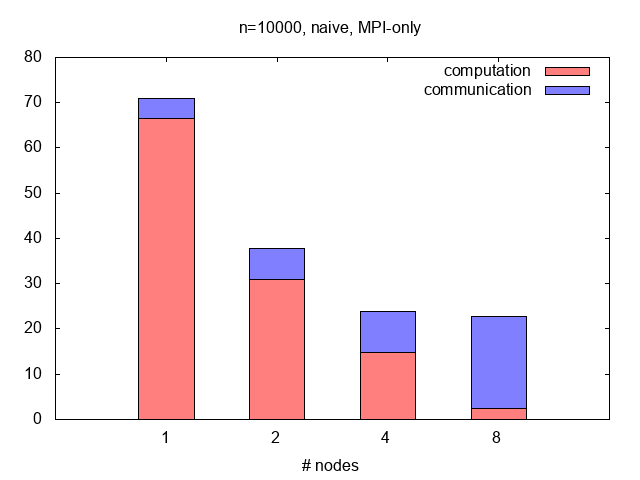
\includegraphics[width=0.43\textwidth]{plot_10000_naive_serial.png} 
	\qquad
	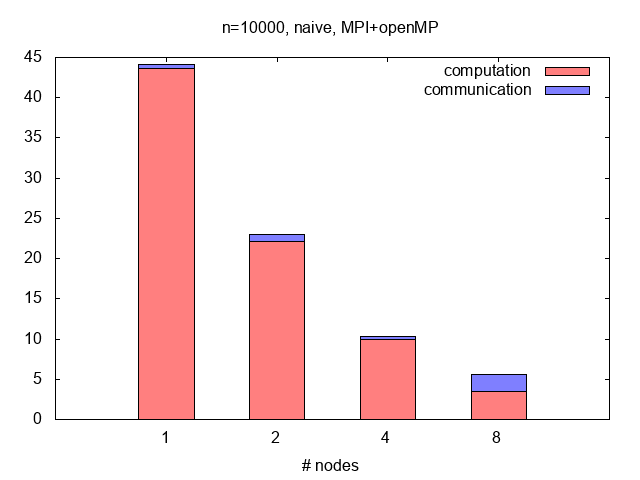
\includegraphics[width=0.43\textwidth]{plot_10000_naive_thread.png} 
	\qquad
	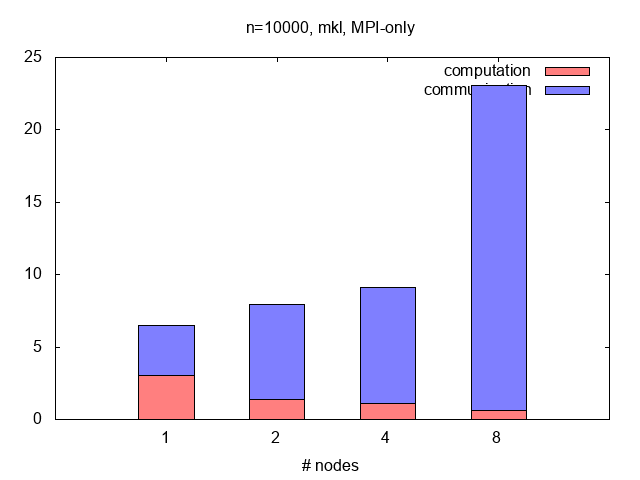
\includegraphics[width=0.43\textwidth]{plot_10000_mkl_serial.png} 
	\qquad
	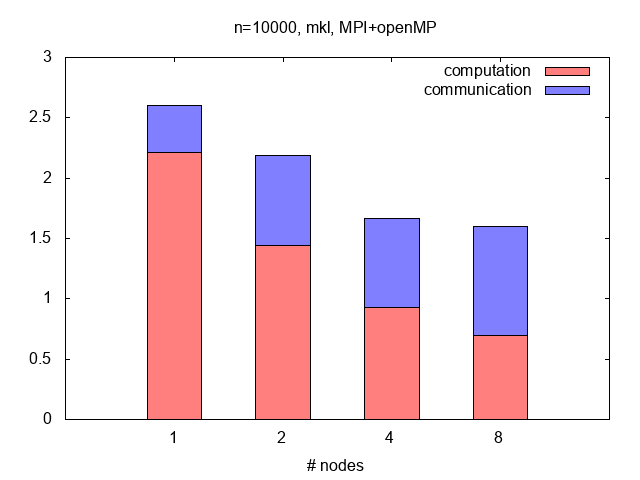
\includegraphics[width=0.43\textwidth]{plot_10000_mkl_thread.png} 
\end{figure}

\begin{figure}[H]
	\centering
	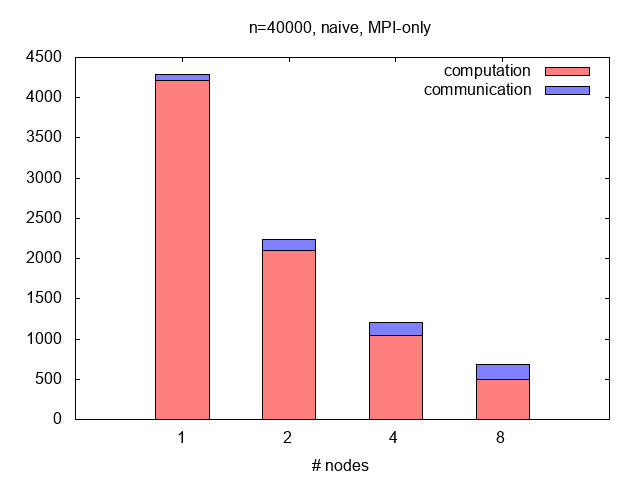
\includegraphics[width=0.43\textwidth]{plot_40000_naive_serial.png} 
	\qquad
	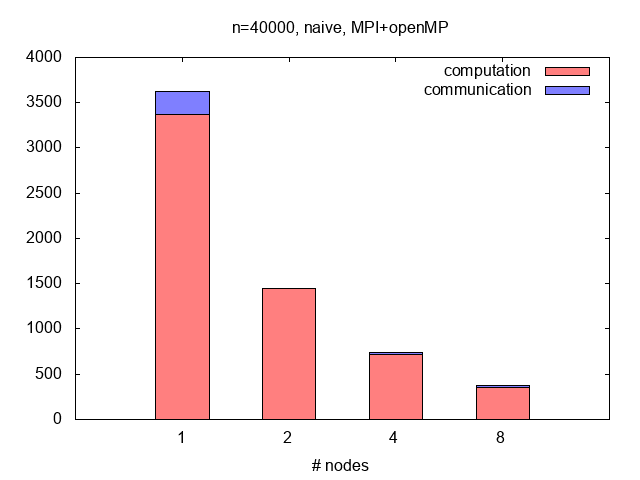
\includegraphics[width=0.43\textwidth]{plot_40000_naive_thread.png} 
	\qquad
	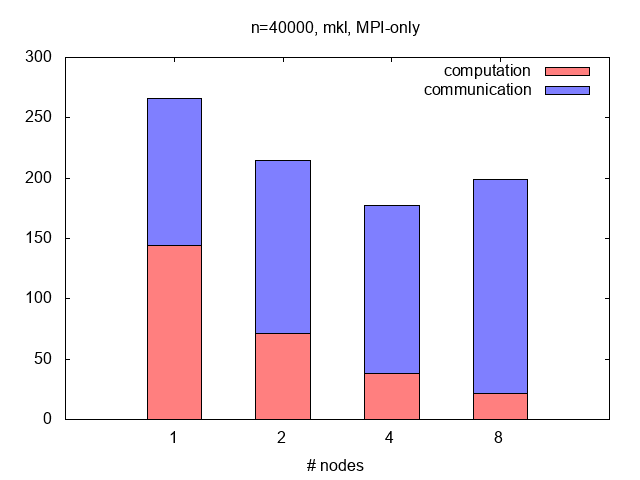
\includegraphics[width=0.43\textwidth]{plot_40000_mkl_serial.png} 
	\qquad
	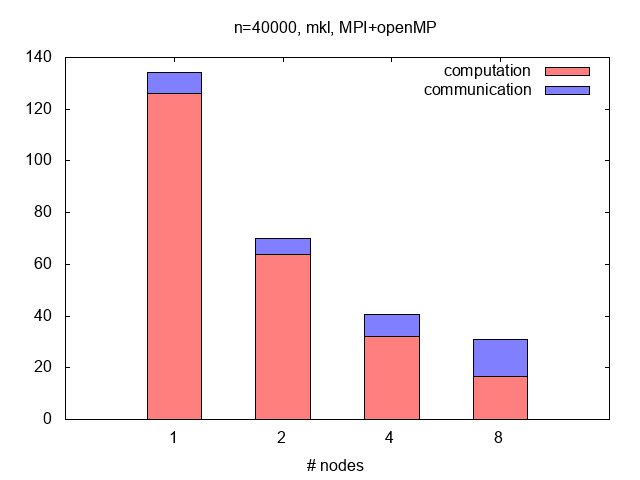
\includegraphics[width=0.43\textwidth]{plot_40000_mkl_thread.png} 
\end{figure}



\section*{Acceleration with Cuda}  % Cuda upgrade
The next step in the exercise was to port the code in Cuda so that the matrix multiplication is offloaded to the GPU. Every GPU is associated to an MPI process with \texttt{cudaSetDevice}.%, so that communication is optimized.

Matrices $A$ and $B$ are initialized on CPU in parallel with OpenMP threads. Matrix $A$ is then transferred to the GPU once before the beginning of the main loop, while $Bloc$ is copied at each iteration. This means that $B$ exists only in the CPU. At the end of the loop, $C$ is copied back to CPU so that the result of the multiplication can be possibly printed by the program.
At each iteration, after performing the \textit{allgather}, every MPI process sends $Bloc$ to the associated GPU with \texttt{cudaMemcpy}, and then a \texttt{cublasDgemm} kernel is launched.

Since \texttt{cublasDgemm} wants matrices in column-major order, the routine was called exchanging $A$ and $B$ in the parameters. This trick exploits the property of transpose matrices that $(AB)^t = B^t A^t$ and the fact that transposing a matrix is equivalent to changing from row-major to column-major order.

The \textit{total} time measured includes transfers of A and C, as well as the main loop. This \textit{total} time is to be compared against the $Tcomm + Tcomp$ of previous section. The $Tcomm$ will obviously be the same. The remaining time (indicated in the plots with \textit{"total - comm."}) comprises computation and CPU-GPU data transfers.
%corresponds to
%The $Tcomp$ now is not directly measured, because 
It is worth pointing out that the initialization of the Cublas handle with \texttt{cublasCreate} takes approximately 0.7 seconds, which was not included in the total time.


The code was compiled with $nvcc$, linking against the MPI and Cublas libraries. Each node in partition \textit{gpu2} of \textit{Ulysses} has 2 GPUs, one per socket, so the program was run using 2 MPI processes per node.% The number of nodes used was 1, 2 and 4.

This new Cuda version was compared with the previous CPU code (the version with mkl and MPI+OpenMP) in terms of execution time (see the plots below).
The memory limitation is now stricter than before, as the GPU memory is smaller than the CPU memory. The largest feasible size of matrix now is roughly $n=37000$ which corresponds to an amount of memory of
\[ 37000^2 \times 3 \times 8\mathrm{B} = 30.6 \mathrm{GB} \]
which can fit in one node having 32 GB (16 GB per GPU).



The double-precision performance of a Tesla P100 (the GPU present on Ulysses) is 4.7 TFlops. There are two GPUs per node, so the compute power per node is 9.4 TFlops, to be compared to the 1.1 TFlops of the CPUs. This larger compute power comes at the price of inevitable data transfers between CPU and GPU.
%It is clear from the plots that 
The advantage is not only the larger number of Flops that the GPU is capable of, but also the fact that we are overlapping communication with computation. In fact, the kernel launch is asynchronous with respect to the host, therefore while the GPU is doing the multiplication the CPU can already start to gather the next $Bloc$, effectively achieving CPU and GPU tasks overlap.

\begin{figure}[H]
	\centering
	\includegraphics[width=0.43\textwidth]{plot_N10000_CPU.png} 
	\qquad
	\includegraphics[width=0.43\textwidth]{plot_N10000_GPU.png} 
	\qquad
	\includegraphics[width=0.43\textwidth]{plot_N37000_CPU.png} 
	\qquad
	\includegraphics[width=0.43\textwidth]{plot_N37000_GPU.png} 
\end{figure}





	
\end{document}